% move all configuration stuff into includes file so we can focus on the content
\documentclass[aspectratio=169,hyperref={pdfpagelabels=false,colorlinks=true,linkcolor=white,urlcolor=blue},t]{beamer}

%%%%%%%%%%%%%%%%%%%%%%%%%%%%%%%%%%%%%%%%%%%%%%%%%%%%%%%%%%%%%%%%%%%%%%%%%%%%%%%%%%
%%%%%%%%%%%%%%%%%%%%%%%%%%%%%%%%%%%%%%%%%%%%%%%%%%%%%%%%%%%%%%%%%%%%%%%%%%%%%%%%%%
% packages
\usepackage{pict2e}
\usepackage{epic}
\usepackage{amsmath,amsfonts,amssymb}
\usepackage{units}
\usepackage{fancybox}
\usepackage[absolute,overlay]{textpos} 
\usepackage{media9} % avi2flv: "C:\Program Files\ffmpeg\bin\ffmpeg.exe" -i TuneFreqFilterbank.avi -b 600k -s 441x324 -r 15 -acodec copy TuneFreqFilterbank.flv
\usepackage{animate}
\usepackage{gensymb}
\usepackage{multirow}
\usepackage{silence}
\usepackage[backend=bibtex,style=ieee]{biblatex}
\AtEveryCitekey{\iffootnote{\tiny}{}}
\addbibresource{references}

%%%%%%%%%%%%%%%%%%%%%%%%%%%%%%%%%%%%%%%%%%%%%%%%%%%%%%%%%%%%%%%%%%%%%%%%%%%%%%%%%%
%%%%%%%%%%%%%%%%%%%%%%%%%%%%%%%%%%%%%%%%%%%%%%%%%%%%%%%%%%%%%%%%%%%%%%%%%%%%%%%%%%
% relative paths
\graphicspath{{graph/}}


%%%%%%%%%%%%%%%%%%%%%%%%%%%%%%%%%%%%%%%%%%%%%%%%%%%%%%%%%%%%%%%%%%%%%%%%%%%%%%%%%%
%%%%%%%%%%%%%%%%%%%%%%%%%%%%%%%%%%%%%%%%%%%%%%%%%%%%%%%%%%%%%%%%%%%%%%%%%%%%%%%%%%
% units
\setlength{\unitlength}{1mm}

%%%%%%%%%%%%%%%%%%%%%%%%%%%%%%%%%%%%%%%%%%%%%%%%%%%%%%%%%%%%%%%%%%%%%%%%%%%%%%%%%%
%%%%%%%%%%%%%%%%%%%%%%%%%%%%%%%%%%%%%%%%%%%%%%%%%%%%%%%%%%%%%%%%%%%%%%%%%%%%%%%%%%
% theme & layout
\usetheme{Frankfurt}
\beamertemplatenavigationsymbolsempty
%\setbeamertemplate{frametitle}[smoothbars theme]
\setbeamertemplate{frametitle}
{
    \begin{beamercolorbox}[ht=1.8em,wd=\paperwidth]{frametitle}
        \vspace{-.1em}%
        \hspace{.2em}{\strut\insertframetitle\strut}
        
        \hspace{.2em}\small\strut\insertframesubtitle\strut
        %\hfill
        %
\includegraphics[height=.8cm,keepaspectratio]{CenterMusicTechnology-solid-2lines-white-CoAtag}
        
    \end{beamercolorbox}
    \begin{textblock*}{100mm}(11.6cm,.7cm)
        \includegraphics[height=.8cm,keepaspectratio]{logo_GTCMT_black}
    \end{textblock*}
}

% set this to ensure bulletpoints without subsections
\usepackage{remreset}
\makeatletter
\@removefromreset{subsection}{section}
\makeatother
\setcounter{subsection}{1}

%---------------------------------------------------------------------------------
% appearance
\setbeamercolor{structure}{fg=gtgold}
\setbeamercovered{transparent} %invisible
\setbeamercolor{bibliography entry author}{fg=black}
\setbeamercolor*{bibliography entry title}{fg=black}
\setbeamercolor*{bibliography entry note}{fg=black}

%\usepackage{pgfpages}
%\setbeameroption{show notes}
%\setbeameroption{show notes on second screen=right}
%---------------------------------------------------------------------------------
% fontsize
\let\Tiny=\tiny

%%%%%%%%%%%%%%%%%%%%%%%%%%%%%%%%%%%%%%%%%%%%%%%%%%%%%%%%%%%%%%%%%%%%%%%%%%%%%%%%%%
%%%%%%%%%%%%%%%%%%%%%%%%%%%%%%%%%%%%%%%%%%%%%%%%%%%%%%%%%%%%%%%%%%%%%%%%%%%%%%%%%%
% warnings
\pdfsuppresswarningpagegroup=1
\WarningFilter{biblatex}{Patching footnotes failed}
\WarningFilter{latexfont}{Font shape}
\WarningFilter{latexfont}{Some font shapes}
\WarningFilter{gensymb}{Not defining}


%%%%%%%%%%%%%%%%%%%%%%%%%%%%%%%%%%%%%%%%%%%%%%%%%%%%%%%%%%%%%%%%%%%%%%%%%%%%%%%%%%
%%%%%%%%%%%%%%%%%%%%%%%%%%%%%%%%%%%%%%%%%%%%%%%%%%%%%%%%%%%%%%%%%%%%%%%%%%%%%%%%%%
% title information
\title[]{Introduction to Audio Content Analysis}   
\author[alexander lerch]{alexander lerch} 
%\institute{~}
%\date[Alexander Lerch]{}
\titlegraphic{\vspace{-16mm}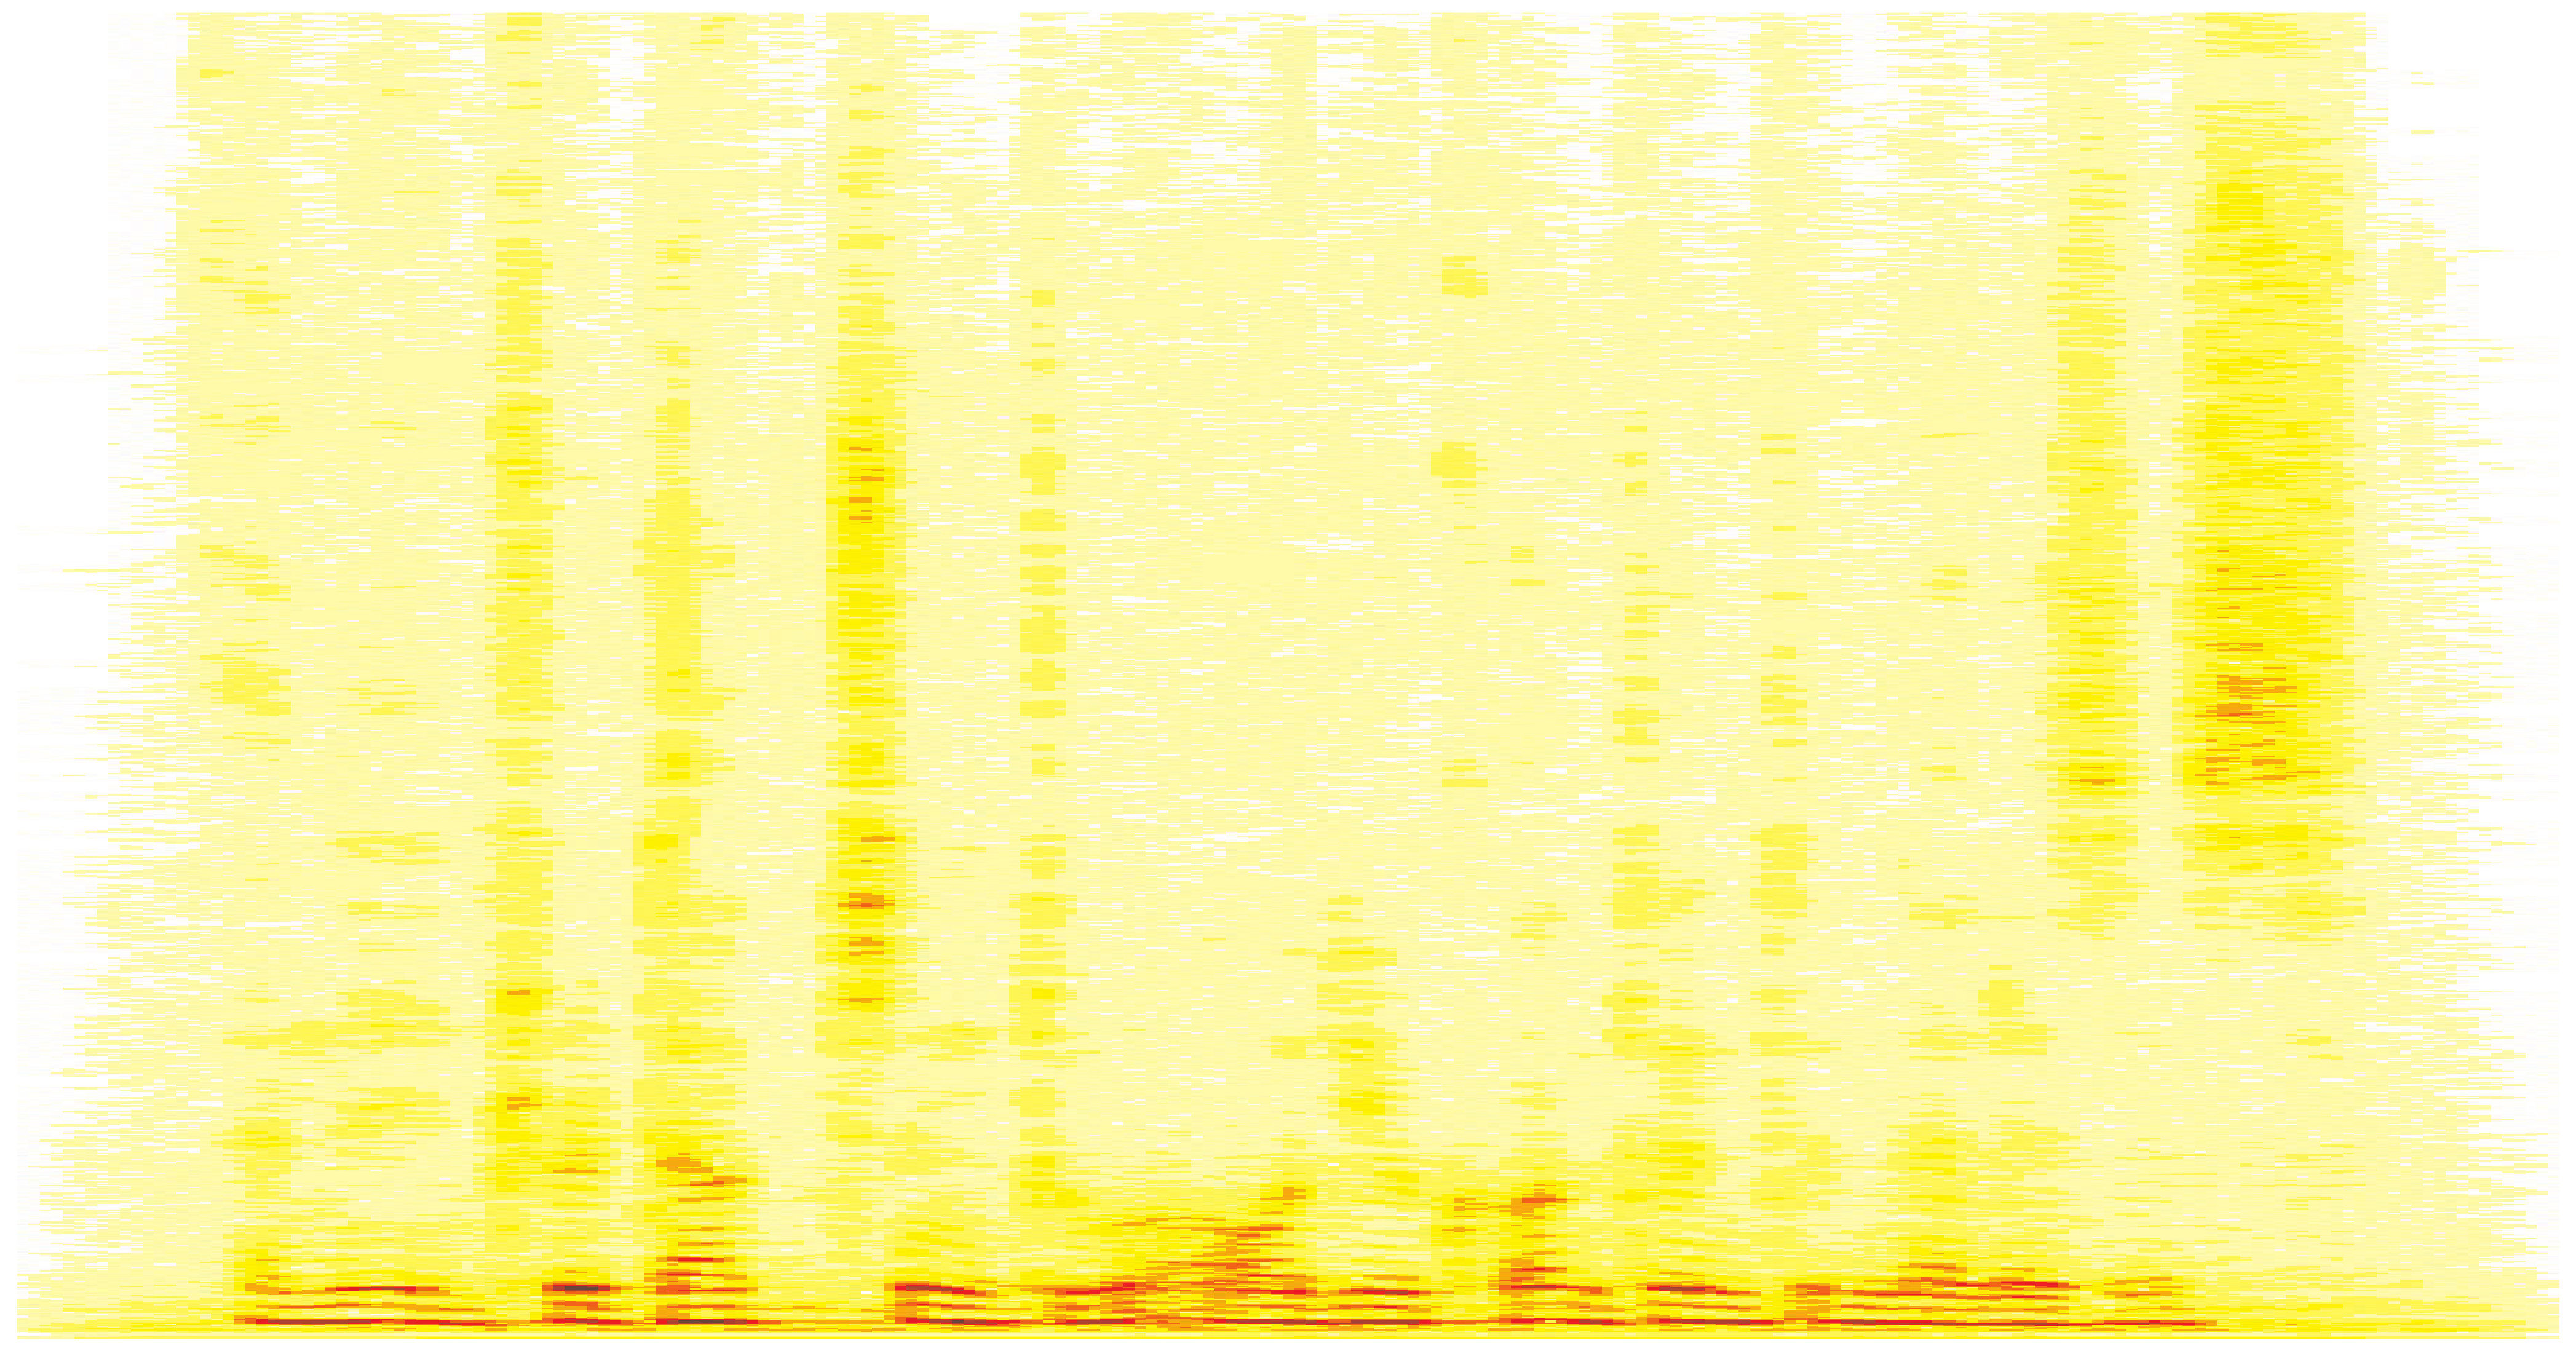
\includegraphics[width=\textwidth,height=3cm]{title}}

%%%%%%%%%%%%%%%%%%%%%%%%%%%%%%%%%%%%%%%%%%%%%%%%%%%%%%%%%%%%%%%%%%%%%%%%%%%%%%%%%%
%%%%%%%%%%%%%%%%%%%%%%%%%%%%%%%%%%%%%%%%%%%%%%%%%%%%%%%%%%%%%%%%%%%%%%%%%%%%%%%%%%
% colors
\definecolor{gtgold}{HTML}{E0AA0F} %{rgb}{0.88,0.66,1,0.06} [234, 170, 0]/256

%%%%%%%%%%%%%%%%%%%%%%%%%%%%%%%%%%%%%%%%%%%%%%%%%%%%%%%%%%%%%%%%%%%%%%%%%%%%%%%%%%
%%%%%%%%%%%%%%%%%%%%%%%%%%%%%%%%%%%%%%%%%%%%%%%%%%%%%%%%%%%%%%%%%%%%%%%%%%%%%%%%%%
% math
\DeclareMathOperator*{\argmax}{argmax}
\DeclareMathOperator*{\argmin}{argmin}
\DeclareMathOperator*{\atan}{atan}
\DeclareMathOperator*{\arcsinh}{arcsinh}
\DeclareMathOperator*{\sign}{sign}
\DeclareMathOperator*{\tcdf}{tcdf}
\DeclareMathOperator*{\si}{sinc}
\DeclareMathOperator*{\princarg}{princarg}
\DeclareMathOperator*{\arccosh}{arccosh}
\DeclareMathOperator*{\hwr}{HWR}
\DeclareMathOperator*{\flip}{flip}
\DeclareMathOperator*{\sinc}{sinc}
\DeclareMathOperator*{\floor}{floor}
\newcommand{\e}{{e}}
\newcommand{\jom}{\mathrm{j}\omega}
\newcommand{\jOm}{\mathrm{j}\Omega}
\newcommand   {\mat}[1]    		{\boldsymbol{\uppercase{#1}}}		%bold
\renewcommand {\vec}[1]    		{\boldsymbol{\lowercase{#1}}}		%bold

%%%%%%%%%%%%%%%%%%%%%%%%%%%%%%%%%%%%%%%%%%%%%%%%%%%%%%%%%%%%%%%%%%%%%%%%%%%%%%%%%%
%%%%%%%%%%%%%%%%%%%%%%%%%%%%%%%%%%%%%%%%%%%%%%%%%%%%%%%%%%%%%%%%%%%%%%%%%%%%%%%%%%
% media9
\newcommand{\includeaudio}[1]{{\includemedia[
                        addresource=audio/#1.mp3,
                        width=5mm,
                        height=5mm,
                        activate=onclick,
                        flashvars={
                            source=audio/#1.mp3  
                            &autoPlay=true
                        }]
                        {
\includegraphics[width=5mm, height=5mm]{SpeakerIcon}}
                        {APlayer.swf}}}
\newcommand{\audioautoplay}[1]{{\begin{center}\includemedia[
                            addresource=audio/#1.mp3,
                            width=.1\linewidth,
                            height=.01\linewidth,
                            activate=pageopen,
                            flashvars={
                                source=audio/#1.mp3  
                                &autoPlay=true
                            }]
                            {}
                            {APlayer.swf}\end{center}}}

\newcommand{\includevideo}[1]{{\begin{center}\includemedia[
                        addresource=video/#1.mp4,
                        width=0.8\linewidth,
                        height=0.4\linewidth,
                        activate=onclick,
                        flashvars={
                            source=video/#1.mp4  
                            &autoPlay=true
                        }]
                        {}
                        {VPlayer.swf}\end{center}}}
\newcommand{\videowithmatlab}[1]{{\begin{center}\includemedia[
                        addresource=video/animate#1.mp4,
                        width=0.8\linewidth,
                        height=0.4\linewidth,
                        activate=onclick,
                        flashvars={
                            source=video/animate#1.mp4  
                            &autoPlay=true
                        }]
                        {}
                        {VPlayer.swf}\end{center}\addreference{matlab source: matlab/animate#1.m}}}
                        

%%%%%%%%%%%%%%%%%%%%%%%%%%%%%%%%%%%%%%%%%%%%%%%%%%%%%%%%%%%%%%%%%%%%%%%%%%%%%%%%%%
%%%%%%%%%%%%%%%%%%%%%%%%%%%%%%%%%%%%%%%%%%%%%%%%%%%%%%%%%%%%%%%%%%%%%%%%%%%%%%%%%%
% other commands
\newcommand{\question}[1]{%\vspace{-4mm}
                          \setbeamercovered{invisible}
                          \begin{columns}[T]
                            \column{.8\textwidth}
                                \textbf{#1}
                            \column{.2\textwidth}
                                \vspace{-8mm}
                                \begin{flushright}
                                     
\includegraphics[scale=.5]{question_mark}
                                \end{flushright}
                                \vspace{6mm}
                          \end{columns}\pause\vspace{-12mm}}

\newcommand{\toremember}[1]{%\vspace{-4mm}
                          \begin{columns}[T]
                            \column{.8\textwidth}
                                \textbf{#1}
                            \column{.2\textwidth}
                                \vspace{-4mm}
                                \begin{flushright}
                                     
\includegraphics[scale=.5]{exclamation_mark}
                                \end{flushright}
                                \vspace{6mm}
                          \end{columns}\vspace{-6mm}}

\newcommand{\matlabexercise}[1]{%\vspace{-4mm}
                          \setbeamercovered{invisible}
                          \begin{columns}[T]
                            \column{.8\textwidth}
                                \textbf{matlab exercise}: #1
                            \column{.2\textwidth}
                                \begin{flushright}
                                     
\includegraphics[scale=.5]{logo_matlab}
                                \end{flushright}
                                %\vspace{6mm}
                          \end{columns}}

\newcommand{\addreference}[1]{  
                  
                    \begin{textblock*}{\baselineskip }(1.12\textwidth,.3\textheight) %(1.15\textwidth,.4\textheight)
                        \rotatebox{90}{\tiny {#1}}
                    \end{textblock*}}
                    
\newcommand{\figwithmatlab}[1]{
                    \begin{figure}
                        \centering
                        \includegraphics{#1}
                        %\label{fig:#1}
                    \end{figure}
                    
                    \addreference{matlab source: \href{https://github.com/alexanderlerch/ACA-Slides/blob/master/matlab/display#1.m}{matlab/display#1.m}}}
\newcommand{\figwithref}[2]{
                    \begin{figure}
                        \centering
                        \includegraphics{#1}
                        \label{fig:#1}
                    \end{figure}
                    
                    \addreference{#2}}  
                                    
\newcommand{\inserticon}[1]{

                    \begin{textblock*}{100mm}(14.5cm,7.5cm)
                        \includegraphics[height=.8cm,keepaspectratio]{#1}
                    \end{textblock*}}            

%%%%%%%%%%%%%%%%%%%%%%%%%%%%%%%%%%%%%%%%%%%%%%%%%%%%%%%%%%%%%%%%%%%%%%%%%%%%%%%%%%
%%%%%%%%%%%%%%%%%%%%%%%%%%%%%%%%%%%%%%%%%%%%%%%%%%%%%%%%%%%%%%%%%%%%%%%%%%%%%%%%%%
% counters
\newcounter{i}
\newcounter{j}
\newcounter{iXOffset}
\newcounter{iYOffset}
\newcounter{iXBlockSize}
\newcounter{iYBlockSize}
\newcounter{iYBlockSizeDiv2}
\newcounter{iDistance}



\subtitle{Module 8.2: Music Similarity}

%%%%%%%%%%%%%%%%%%%%%%%%%%%%%%%%%%%%%%%%%%%%%%%%%%%%%%%%%%%%%%%%%%%%%%%%%%%%
\begin{document}
    % generate title page
	

\begin{frame}
    \titlepage
    %\vspace{-5mm}
    \begin{flushright}
        \href{http://www.gtcmt.gatech.edu}{\includegraphics[height=.8cm,keepaspectratio]{logo_GTCMT_black}}
    \end{flushright}
\end{frame}


    \section[overview]{lecture overview}
        \begin{frame}{introduction}{overview}
            \begin{block}{corresponding textbook section}
                    \href{http://ieeexplore.ieee.org/xpl/articleDetails.jsp?arnumber=6331125}{Chapter 8: Musical Genre, Similarity, and Mood} (pp.~156--157)
            \end{block}

            \begin{itemize}
                \item   \textbf{lecture content}
                    \begin{itemize}
                        \item   music similarity and its relation to musical genre
                        \item   clustering and visualization of feature space
                    \end{itemize}
                \bigskip
                \item<2->   \textbf{learning objectives}
                    \begin{itemize}
                        \item   describe potential issues with algorithms for measuring music similarity
                        \item   implement a simple k-Means algorithm
                    \end{itemize}
            \end{itemize}
            \inserticon{directions}
        \end{frame}

    \section[intro]{introduction}
        \begin{frame}{music similarity}{introduction}
            \begin{itemize}
                \item	genre classification is just a grouping by specific interpretation of similarity
                    \begin{itemize}
                        \item	similar set of features
                        \item	ambiguous 'ground truth'
                        \item   unclear value/impact of low level and high level features
                    \end{itemize}
                \bigskip
                \item<2->	 \textbf{differences} to genre classification
                    \begin{itemize}
                        %\item	\textit{mood}: often not a classification but regression
                        \item	\textit{similarity}: distance measure instead of categorizing into classes
                    \end{itemize}
            \end{itemize}
        \end{frame}


    \section[similarity]{audio similarity}
        \begin{frame}{audio similarity}{introduction}
            \begin{itemize}
                \item   \textbf{perception} of music similarity
                    \begin{itemize}
                        \item	multi-dimensional (melodic, rhythmic, sound quality, \ldots)
                        \item	user dependent
                        \item	associative, may also depend on editorial data
                        \item	may be context dependent
                    \end{itemize}
                \bigskip
                \item<2->   genres are \textbf{clusters of musical similarity}
                \item<2->[$\Rightarrow$]	genre classification is a \textit{special case} of audio similarity measures
                \item<3->	instead of assigning (genre) labels, the similarity/distance between (pairs) of files is measured
            \end{itemize}
        \end{frame}
    \section{clustering}
        \begin{frame}{audio similarity}{K-Means clustering example}
            \begin{itemize}
                \item   simple k-means example
                    \begin{itemize}
                        \item   \textbf{goal}: minimize intra-cluster variance
                        \item   \textbf{distance}: Euclidean
                        \item   \textbf{procedure}:
                            \begin{enumerate}
                                \item	\textit{initialization}:\\ randomly select $K$ points in the feature space as initialization.
                                \item<2->	\textit{assignment}:\\ assign each observation to the cluster with the mean/centroid of the closest cluster.
                                \item<3->	\textit{update}:\\ compute mean/centroid for each cluster.
                                \item<4->	\textit{iteration}:\\ go to step $2$ until the clusters converge.
                            \end{enumerate}
                    \end{itemize}
            \end{itemize}
        \end{frame}
        \begin{frame}{audio similarity}{K-Means clustering example}
            \begin{columns}
            \column{.5\linewidth}
                    \begin{itemize}
                        \item<1->   data points
                        \item<2->   init randomly
                        \item<3->   iteration
                            \begin{itemize}
                                \item   assign data points to closest centroid
                                \item   update centroids
                            \end{itemize}
                        \item<7->   terminate when convergence
                    \end{itemize}
            \column{.5\linewidth}
            \setcounter{i}{0}
            \setcounter{j}{1}
            \whiledo{\value{i}<7}
            {
                %\only<\value{j}>{\figwithref{KMeans-\arabic{i}}{matlab source: matlab/displayKMeans.m}}
                \only<\value{j}>{\begin{figure}\includegraphics{KMeans-\arabic{i}}\end{figure}}
                \stepcounter{i}
                \stepcounter{j}
            }
            \end{columns}
            \addreference{matlab source: \href{https://github.com/alexanderlerch/ACA-Slides/blob/master/matlab/displayKMeans.m}{matlab/displayKMeans.m}}
        \end{frame}
        \begin{frame}{audio similarity}{visualization in a 2D space}
            \begin{itemize}
                \item \textbf{problem}
                    \begin{itemize}
                        \item   feature space is high-dimensional
                        \item[$\rightarrow$] cannot be visualized
                    \end{itemize}
                \bigskip
                \item<2-> find \textbf{mapping} to 2D ``preserving'' (high-dimensional) distance metrics
                \item[]     examples:
                    \begin{itemize}
                        \item   Self-Organizing Maps
                    \end{itemize}
            \end{itemize}
        \end{frame}
            
        \begin{frame}{audio similarity}{visualization example: SOM 1/2}
            \vspace{-3mm}
                    \begin{enumerate}
                        \item	create a map with 'neurons'
                        \item<1->	train
                                \begin{itemize}
                                    \item	for each training sample find BMU (best matching unit)
                                    \item	adapt BMU and neighbors toward training sample
                                    \begin{equation*}
                                        W_v(t + 1) = W_v(t) + \theta (v, t) \alpha(t)\big(D(t) - W_v(t)\big)
                                    \end{equation*}
                                    \begin{footnotesize}
                                        \begin{itemize}
                                            \item	$\theta (v, t)$: depends on distance from BMU
                                            \item	$\alpha (t)$: learning restraint
                                            \item	$D(t)$ training sample
                                        \end{itemize}
                                    \end{footnotesize}
                                \end{itemize}
                    \end{enumerate}
                    \only<1->{
                    \begin{figure}
                        \centering
                            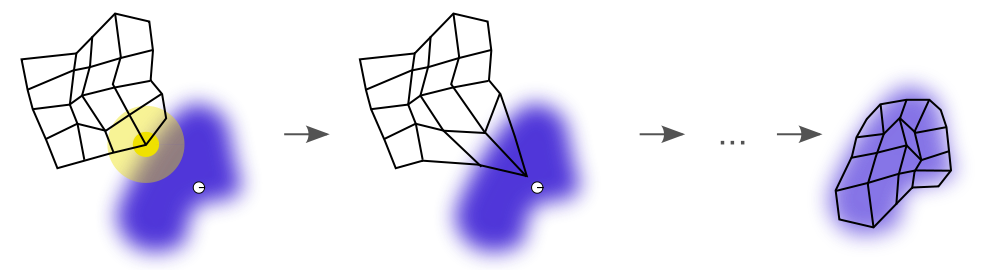
\includegraphics[scale=.3]{graph/SOM_training}
                    \end{figure}
                    \addreference{\url{https://en.wikipedia.org/wiki/Self-organizing_map}}}
        \end{frame}
        \begin{frame}{audio similarity}{SOM 2/2}
            \vspace{-2mm}
            \begin{figure}
                \centering
                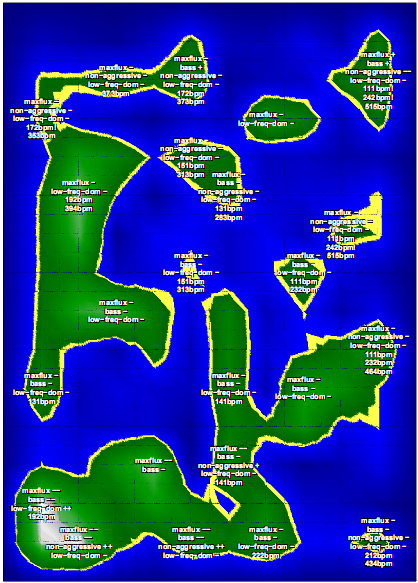
\includegraphics[scale=.28]{graph/som}
            \end{figure}
            \vspace{-10mm}from \footfullcite{pampalk_islands_2001}
        \end{frame}
    
    \section{summary}
        \begin{frame}{summary}{lecture content}
            \begin{itemize}
                \item   \textbf{music similarity}
                    \begin{itemize}
                        \item   even less clearly defined than music genre
                    \end{itemize}
                \bigskip
                \item   \textbf{processing steps}
                    \begin{enumerate}
                        \item   extract features
                        \item   define some distance metric in feature space
                    \end{enumerate}
                \bigskip
                \item   \textbf{clustering algorithms}
                    \begin{itemize}
                        \item   work to a certain degree with traditional features
                    \end{itemize}
            \end{itemize}
            \inserticon{summary}
        \end{frame}
\end{document}
